
\begin{frame}{Semana 2 (16/02/2023) - T1P1}
        $X$ e $Y$ son dos esferas de metal sin carga sobre soportes aislantes y están en contacto entre sí. Una barra R cargada positivamente se acerca a $X$ como se muestra en la figura (a).
        
        La esfera $Y$ ahora se aleja de $X$, como en la figura (b).
        
        ¿Cuáles son los estados de carga finales de $X$ e $Y$?
        
        \begin{figure}
            \centering
            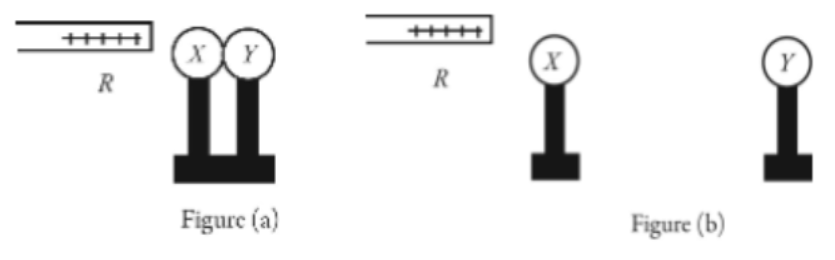
\includegraphics[scale=0.3]{figures/f1.png}
        \end{figure}
        
        \begin{columns}
        \column{0.5\textwidth}
        \begin{itemize}
            \item[A)] Tanto $X$ como $Y$ son neutros.
            \item[B)] $X$ es positivo e $Y$ es neutro.
            \item[C)] $X$ es neutro e $Y$ es positivo.
            \end{itemize}
        \column{0.5\textwidth}
        \begin{itemize}
            \item[D)] $X$ es negativo y $Y$ es positivo.
            \item[E)] Tanto $X$ como $Y$ son negativos.
        \end{itemize}
        \end{columns}
        
        
        
        \pause\bigskip\centering \textbf{Respuesta:} D.
\end{frame}

\begin{frame}{Semana 2 (16/02/2023) - T1P2}
    
    Una carga puntual positiva $Q$ está fija sobre una mesa horizontal muy grande sin fricción. Una segunda carga puntual positiva $q$ se libera desde el reposo cerca de la carga estacionaria y puede moverse libremente. ¿Qué enunciado describe mejor el movimiento de $q$ después de que se suelta?
    
    \begin{itemize}
    
    \item[A)]Su velocidad será máxima justo después de que se suelte.

    \item[B)] Su aceleración es cero justo después de que se suelta.
    
    \item[C)] A medida que se aleja más y más de $Q$, su aceleración seguirá aumentando.
    
    \item[D)] A medida que se aleja más y más de $Q$, su velocidad disminuirá.
    
    \item[E)] A medida que se aleja más y más de $Q$, su velocidad seguirá aumentando.
    \end{itemize}
    
    \pause\bigskip\centering\textbf{Respuesta:} E.
    
\end{frame}

\begin{frame}{Semana 2 (16/02/2023)- T1P3}
    
    Una bola de plástico muy pequeña cargada uniformemente está ubicada directamente encima de otra carga similar en un tubo de ensayo como se muestra en la figura. Las bolas están en equilibrio a una distancia $d$.
    
    \begin{columns}
    \column{0.5\textwidth}
     \begin{figure}
        \centering
        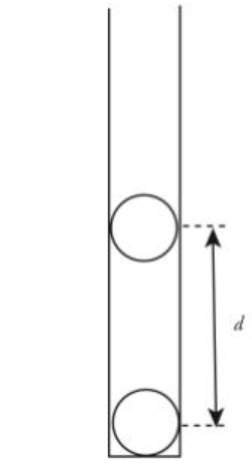
\includegraphics[scale=0.3]{figures/p2.png}
    \end{figure}
    
    \column{0.5\textwidth}

Si se duplica la carga de cada bola, la distancia entre las bolas en el tubo de ensayo sería
    
     \begin{itemize}
        \item[A)] $\sqrt{2}d$
        \item[B)] $2d$
        \item[C)] $4d$
        \item[D)] $8d$
    \end{itemize}
    
    \pause\bigskip\centering\textbf{Respuesta:} B.

    \end{columns}
    
\end{frame}

\begin{frame}{Semana 2 (16/02/2023)- T1P4}
    
    En la figura, $Q = 5.8$ nC. ¿Cuál es la magnitud de la fuerza el\'ectrica sobre la carga $Q$?
    
    \begin{figure}
        \centering
        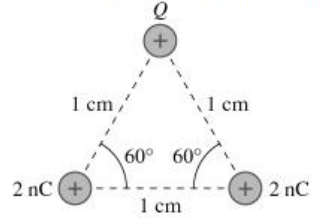
\includegraphics[scale=0.5]{figures/f3.png}
    \end{figure}
    
\end{frame}

\begin{frame}{Semana 2 (16/02/2023)- T1P5}
    Cuatro cargas puntuales negativas iguales están ubicadas en las esquinas de un cuadrado, sus posiciones en el plano $xy$ son $(1, 1)$, $(-1, 1)$, $(-1, -1)$ y $(1, -1)$. Si se posiciona una carga positiva en el punto $(1,0)$, determine la direcci\'on de la fuerza el\'ectrica que esta experimenta.
\end{frame}

\begin{frame}{Semana 2 (16/02/2023)- T1P6}
    
    Determine la magnitud y direcci\'on de la fuerza el\'ectrica que experimenta una carga puntual positiva $q$ ubicada en el punto $(L,d)$, debida a una barra delgada cargada homogéneamente con una carga $Q$ negativa y que est\'a sobre el eje $x$ en $0\leq x\leq L$.
    
\end{frame}

\begin{frame}{Semana 2 (16/02/2023)- Q1}
    
    La figura muestra dos diminutas esferas de masa $m$ que est\'an suspendidas de dos hilos muy delgados de longitud $L$. Las esferas se repelen entre sí después de cargarse con la misma magnitud de carga $Q$ y cuelgan en reposo como se muestra en la figura. ¿Cuál es valor del ángulo $\theta$?
    
    \begin{figure}
        \centering
        \includegraphics[scale=0.4]{figures/Q1.png}
    \end{figure}
    
\end{frame}

\begin{frame}{Semana 3 (22/02/2023) - T2P1}

    La figura muestra tres cargas eléctricas etiquetadas como $Q_1$, $Q_2$, $Q_3$ y algunas líneas de campo eléctrico en la región que rodea las cargas.
    
    \begin{figure}[H]
        \centering
        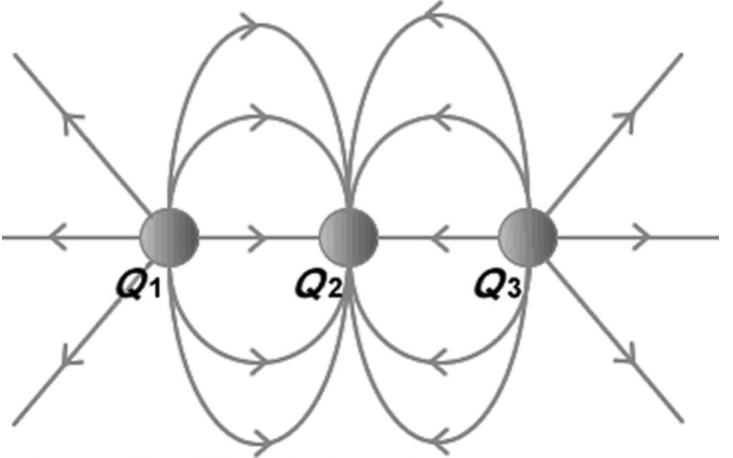
\includegraphics[scale=0.2]{figures/t2p1.png}
    \end{figure}
    
    ¿Cuáles son los signos de las tres cargas?
    
    \begin{columns}
    \column{0.5\textwidth}
    \begin{itemize}
        \item[A)] $Q_1$ es positivo, $Q_2$ es negativo y $Q_3$ es positivo.
        \item[B)] $Q_1$ es negativo, $Q_2$ es positivo y $Q_3$ es negativo.
    \end{itemize}
    \column{0.5\textwidth}
    \begin{itemize}
        \item[C)] $Q_1$ es positivo, $Q_2$ es positivo y $Q_3$ es negativo.
        \item[D)] Las tres cargas son negativas.
        \item[E)] Las tres cargas son positivas.
    \end{itemize}
    
    \end{columns}
    
    \pause\bigskip\centering\textbf{Respuesta:} A.
    
\end{frame}

\begin{frame}{Semana 3 (22/02/2023) - T2P2}

    Un electrón se mueve inicialmente hacia la derecha cuando entra en un campo eléctrico uniforme dirigido hacia arriba.
    
    \begin{figure}
        \centering
        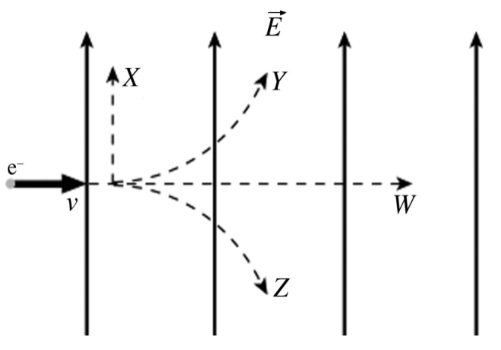
\includegraphics[scale=0.3]{figures/t2p2.png}
    \end{figure}
    
    ¿Cuál de las trayectorias mostradas seguirá el electrón?
    
    \begin{columns}
    \column{0.2\textwidth}
    
    \begin{itemize}
        \item[A)] W.
        \item[B)] X.
    \end{itemize}
    
    \column{0.2\textwidth}
    
    \begin{itemize}
        \item[C)] Y.
        \item[D)] Z.
    \end{itemize}
    
    \column{0.2\textwidth}
    \pause\centering\textbf{Respuesta:} D.
    \end{columns}
    
\end{frame}

\begin{frame}{Semana 3 (22/02/2023) - T2P3}

    Un dipolo eléctrico inicialmente estacionario de momento dipolar $\Vec{p}=\left(5.0\times10^{-10}\text{ C}\cdot\text{m }\right)\hat{\imath},$ es colocado en un campo eléctrico $\vec{E}=\left( 2.00\times10^6\text{ N/C} \right)\left(\hat{\imath}+\hat{\jmath}\right)$ ¿Cuál es la magnitud del torque máximo que el campo eléctrico ejerce sobre el dipolo?
    
\end{frame}

\begin{frame}{Semana 3 (22/02/2023) - T2P4}

    Un dipolo eléctrico consta de cargas $\pm Q$ separadas una distancia $d$. Está colocado en un campo eléctrico vertical de magnitud $E$ orientado como se muestra en la figura.
    
    \begin{columns}
    \column{0.5\textwidth}
    
    \begin{figure}
        \centering
        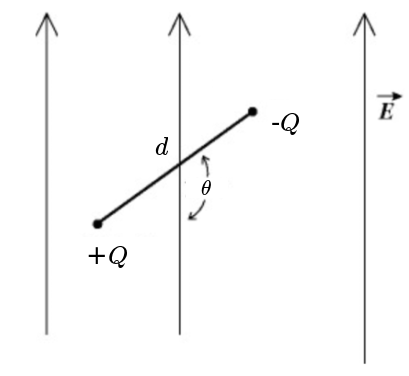
\includegraphics[scale=0.35]{figures/t2p4.png}
    \end{figure}
    
    \column{0.5\textwidth}
    
    La magnitud del torque neto que este campo ejerce sobre el dipolo est\'a dada por
    
    \begin{itemize}
        \item[A)] $QEd\sin\theta$.
        \item[B)] $\frac{QE}{2}d\cos\theta$.
        \item[C)] $QEd\cos\theta$.
        \item[D)] $\frac{QE}{2}d\sin\theta$.
    \end{itemize}
    
    \pause\bigskip\centering\textbf{Respuesta:} A.
    
    \end{columns}
    
\end{frame}

\begin{frame}{Semana 3 (22/02/2023) - T2P5}
    
    Determine la magnitud y direcci\'on de la fuerza el\'ectrica que experimenta una carga puntual positiva $q$ ubicada en el punto $(L,d)$, debida a una barra delgada cargada homogéneamente con una carga $Q$ negativa y que est\'a sobre el eje $x$ en $0\leq x\leq L$.
    
\end{frame}

\begin{frame}{Semana 3 (22/02/2023) - T2P6}

Un semicírculo de radio $a$ se encuentra en los cuadrantes primero y segundo, y con el centro de curvatura en el origen. La carga positiva $+Q$ está distribuida de manera uniforme alrededor de la mitad izquierda del semicírculo, y la carga negativa $-Q$ está distribuida de manera uniforme
alrededor de la mitad derecha del semicírculo como lo muestra la figura.

\begin{figure}
    \centering
    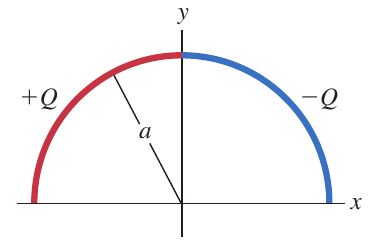
\includegraphics[scale=0.3]{figures/t2p6.png}
\end{figure}

¿Cuál es la magnitud y dirección del campo eléctrico neto en el origen generado por esta distribución de carga?
    
\end{frame}

\begin{frame}{Semana 3 (22/02/2023) - T2P7 (Bonus)}
    Considere dos alambres delgados que est\'an sobre el eje $x$. El primero se encuentra en $-d/2<x<-d/2-L$ y el segundo en $d/2<x<d/2+L$. Cada uno tiene longitud $L$ y posee carga positiva $Q$ distribuida uniformemente.
    
    \begin{itemize}
        \item[a)] Determine el campo el\'ectrico que el primer alambre genera sobre el eje $x$ positivo.
        \item[b)] Demuestre que la magnitud de la fuerza el\'ectrica que un alambre ejerce sobre el otro est\'a dada por
        
        \begin{equation}
            F=\frac{1}{4\pi\epsilon_0}\left(\frac{Q}{L}\right)^2\ln\left[\frac{\left(d+L\right)^2}{d(d+2L)}\right]
        \end{equation}
        
        \item[c)] Demuestre que si $L>>d$, entonces
        
        \begin{equation}
            F=\frac{1}{4\pi\epsilon_0}\left(\frac{Q}{d}\right)^2.
        \end{equation}
        
    \end{itemize}

\end{frame}

\begin{frame}{Semana 3 (22/02/2023) - Q2}
    
    Dos alambres no conductores de longitud $L$ cada uno, forman un ángulo recto. Un segmento tiene una carga neta de $-Q$, distribuida de modo uniforme por toda su longitud; el otro segmento tiene tiene una carga neta de $+Q$, distribuida de modo uniforme por toda su longitud, como se ilustra en la figura.
    
    \begin{columns}
    
    \column{0.5\textwidth}
    
    \begin{figure}
        \centering
        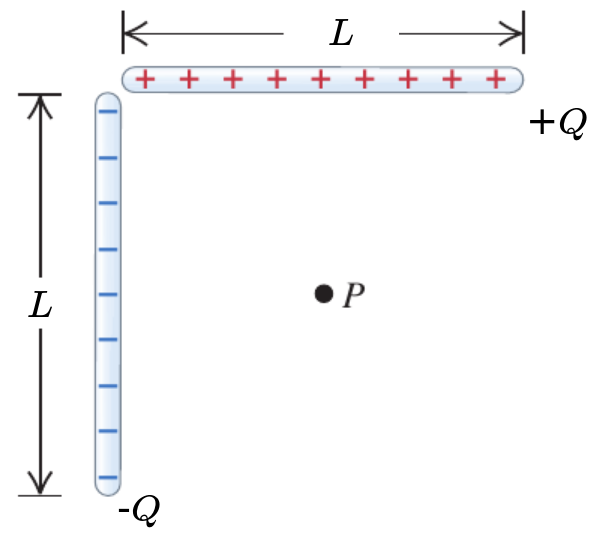
\includegraphics[scale=0.25]{figures/q2.png}
    \end{figure}
    
    \column{0.5\textwidth}
    
    \begin{itemize}
        \item[a)] Determine la magnitud y direcci\'on del campo el\'ectrico que producen estos alambres en el punto $P$, que dista $L/2$ de cada alambre. 
        \item[b)] Si un electr\'on se libera en $P$, ¿cuál es la magnitud y dirección de la fuerza neta que ejercen estos alambres sobre él?
    \end{itemize}
    
    \end{columns}
    
\end{frame}

\begin{frame}{Semana 4 (02/03/2023) - T3P1}
    
    La figura muestra cuatro superficies gaussianas que rodean una distribución de cargas puntuales.
    
    \begin{figure}
        \centering
        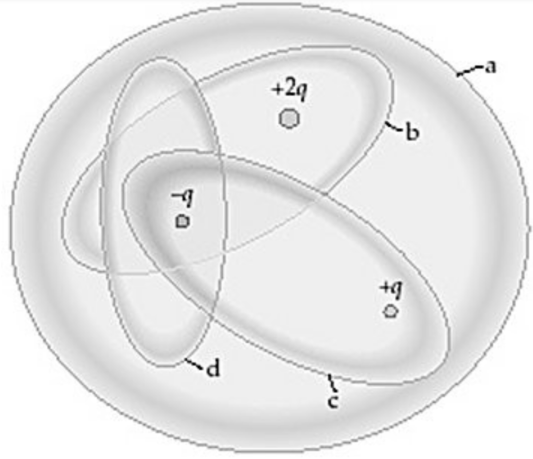
\includegraphics[scale=0.25]{figures/t3p1.png}
    \end{figure}
    
    \begin{itemize}
        \item[a)] ¿Qué superficies gaussianas tienen un flujo eléctrico de $+q/\epsilon_0$ a través de ellas? 
        \pause \textbf{Respuesta:} b
        \pause \item[b)] ¿Qué superficies gaussianas no tienen flujo eléctrico a través de ellas? 
        \pause \textbf{Respuesta:} c
    \end{itemize}
    
\end{frame}

\begin{frame}{Semana 4 (02/03/2023) - T3P2}
    
    ¿Cuáles de las siguientes afirmaciones sobre la ley de Gauss son correctas? (Puede haber más de una opción correcta).
    
    \begin{itemize}
        \item[A)] La ley de Gauss es válida solo para distribuciones de carga simétricas, como esferas y cilindros.

        \item[B)] Si no hay carga dentro de una superficie gaussiana, el campo eléctrico debe ser cero en los puntos de esa superficie.
        
        \item[C)] Solo la carga encerrada dentro de una superficie gaussiana puede producir un campo eléctrico en puntos de esa superficie.
        
        \item[D)] Si una superficie gaussiana está completamente dentro de un conductor electrostático, el campo eléctrico siempre debe ser cero en todos los puntos de esa superficie.
        
        \item[E)] El flujo eléctrico que pasa a través de una superficie gaussiana depende únicamente de la cantidad de carga dentro de esa superficie, no de su tamaño o forma.
    \end{itemize}
    
    \pause\bigskip\centering\textbf{Respuesta:} D y E.
    
\end{frame}

\begin{frame}{Semana 4 (02/03/2023) - T3P3}
    \begin{columns}
    \column{1.1\textwidth}
    \footnotesize
    
    El gráfico de la figura muestra la intensidad del campo eléctrico en función de la distancia desde el centro de un par de esferas concéntricas uniformemente cargadas. 
    ¿Cuál de las siguientes situaciones podría representar plausiblemente el gráfico? (Puede haber más de una opción correcta).
    \vspace{-2em}
    \begin{figure}
        \centering
        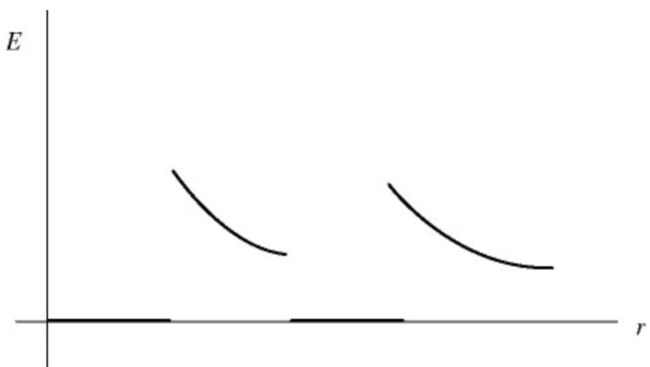
\includegraphics[scale=0.2]{figures/t3p3.png}
    \end{figure}
    \vspace{-2em}
    \begin{itemize}
        \item[A)] Una esfera conductora cargada positivamente dentro de otra esfera conductora cargada positivamente.
        \item[B)] Una esfera conductora cargada positivamente dentro de una esfera conductora sin carga.
        \item[C)] Una esfera sólida no conductora, uniformemente cargada en todo su volumen, dentro de una esfera conductora cargada positivamente.
        \item[D)] Una capa esférica de pared delgada no conductora cargada positivamente dentro de una esfera conductora cargada positivamente.
        \item[E)] Una capa esférica de pared delgada no conductora cargada positivamente dentro de otra capa esférica de pared delgada no conductora cargada positivamente.
    \end{itemize}
    \pause \centering\textbf{Respuesta:} A y D.
    
    \end{columns}

\end{frame}

\begin{frame}{Semana 4 (02/03/2023) - T3P4}
    
    A una distancia $d$ de una línea de carga uniforme muy larga (esencialmente infinita), la intensidad del campo eléctrico es $E$. ¿A qué distancia de la línea la intensidad del campo será $2E$?
    
    \begin{columns}
    \column{0.4\textwidth}
    \begin{itemize}
        \item[A)] $2d$
        \item[B)] $\sqrt{2}d$
        \item[C)] $d/\sqrt{2}$
        \item[D)] $d/2$
        \item[E)] $d/4$
    \end{itemize}
    \column{0.5\textwidth}
    \pause\centering\textbf{Respuesta:} C.
    \end{columns}
    
\end{frame}

\begin{frame}{Semana 4 (02/03/2023) - T3P5}
    
    Una capa esférica no conductora de radio interior $R_1$ y radio exterior $R_2$ contiene una densidad de carga volum\'etrica uniforme $\rho$ en toda la capa. Use la ley de Gauss para derivar una ecuación para la magnitud del campo eléctrico a las siguientes distancias radiales $r$ desde el centro de la esfera. Exprese las respuestas deben estar en términos de $\rho$, $R_1$, $R_2$, $r$, $\epsilon_0$ y $\pi$.
    
    \begin{itemize}
        \item[a)] $r<R_1$
        \item[b)] $R_1<r<R_2$
        \item[c)] $r>R_2$
    \end{itemize}
    
    \pause\textbf{Respuestas:} 
    \begin{columns}
    \column{0.2\textwidth}
    \begin{itemize}
        \item[a)] $E=0$.
    \end{itemize}
    \column{0.4\textwidth}
    \begin{itemize}
        \item[b)] $E=\frac{\rho}{3\epsilon_0 r^2}\left(r^3-R_1^3\right)$.
    \end{itemize}
    \column{0.4\textwidth}
    \begin{itemize}
        \item[c)] $E=\frac{\rho}{3\epsilon_0 r^2}\left(R_2^3-R_1^3\right)$.
    \end{itemize}
    \end{columns}
    
\end{frame}

\begin{frame}{Semana 4 (02/03/2023) - T3P6}
    
    Considere una placa infinita no conductora de espesor $a$, cargada uniformemente con una densidad volum\'etrica de carga $\rho$. Determine la magnitud del campo el\'ectrico en
    
    \begin{itemize}
        \item[a)] Un punto fuera de la placa.
        \item[b)] Un punto en el interior de la placa.
    \end{itemize}
    
\end{frame}

\begin{frame}{Semana 4 (02/03/2023) - T3P7}
    
    Considere dos placas metálicas paralelas muy próximas entre sí y con cargas opuestas. Las placas son cuadradas con lados de longitud $L$ y llevan cargas $Q$ y $-Q$ en sus superficies enfrentadas. ¿Cuál es la magnitud del campo eléctrico en la región entre las placas?
    
    \begin{itemize}
        \item[A)] $E = \frac{Q}{\epsilon_0L^2}$
        \item[B)] $E = \frac{2Q}{\epsilon_0L^2}$.
        \item[C)] $E=0$.
        \item[D)] $E = \frac{4Q}{\epsilon_0L^2}$.
        \item[E)] $E = \frac{Q}{2\epsilon_0L^2}$.
    \end{itemize}
    
    \pause\bigskip\centering\textbf{Respuesta:} A.
    
\end{frame}

\begin{frame}{Semana 4 (02/03/2023) - Q3}
  
  Dos alambres no conductores de longitud $L=\infty$ cada uno, forman un ángulo recto. Un segmento tiene una carga neta de $-Q$, distribuida de modo uniforme por toda su longitud; el otro segmento tiene tiene una carga neta de $+Q$, distribuida de modo uniforme por toda su longitud, como se ilustra en la figura.
    
    \begin{columns}
    
    \column{0.5\textwidth}
    
    \begin{figure}
        \centering
        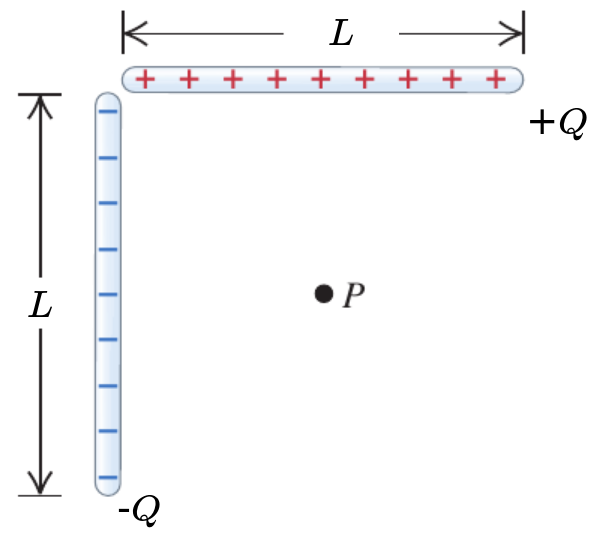
\includegraphics[scale=0.25]{figures/q2.png}
    \end{figure}
    
    \column{0.5\textwidth}
    
    Aplique la ley de gauss para determinar la magnitud del campo el\'ectrico que produce cada alambre en el punto $P$, que dista $L/2$ de cada alambre. Luego, deduzca las direcciones de cada campo y determine el campo el\'ectrico total en $P$.
    
    \end{columns}
    
\end{frame}

\begin{frame}{Semana 5 (09/03/2023) - T4P1}
    
    If the electric field is zero everywhere inside a region of space, the potential must also be zero in that region.
    
    \begin{itemize}
        \item[A)] True.
        \item[B)] False.
    \end{itemize}
    
    
    When the electric field is zero at a point, the potential must also be zero there.
    
    \begin{itemize}
        \item[A)] True.
        \item[B)] False.
    \end{itemize}
    
    If the electrical potential in a region is constant, the electric field must be zero everywhere in that region.
    
    \begin{itemize}
        \item[A)] True.
        \item[B)] False.
    \end{itemize}
    
    f the electric potential at a point in space is zero, then the electric field at that point must also be zero.
    
    \begin{itemize}
        \item[A)] True.
        \item[B)] False.
    \end{itemize}
    
\end{frame}

\begin{frame}{Semana 5 (09/03/2023) - T4P1}
    
    If the electric field is zero everywhere inside a region of space, the potential must also be zero in that region.
    
    \begin{itemize}
        \item[A)] True.
        \item[B)] False. $\leftarrow$ \textbf{Answer}
    \end{itemize}
    
    
    When the electric field is zero at a point, the potential must also be zero there.
    
    \begin{itemize}
        \item[A)] True.
        \item[B)] False. $\leftarrow$ \textbf{Answer}
    \end{itemize}
    
    If the electrical potential in a region is constant, the electric field must be zero everywhere in that region.
    
    \begin{itemize}
        \item[A)] True. $\leftarrow$ \textbf{Answer}
        \item[B)] False.
    \end{itemize}
    
    If the electric potential at a point in space is zero, then the electric field at that point must also be zero.
    
    \begin{itemize}
        \item[A)] True.
        \item[B)] False. $\leftarrow$ \textbf{Answer}
    \end{itemize}
    
\end{frame}

\begin{frame}{Semana 5 (09/03/2023) - T4P2}
    Una esfera metálica de 5 cm de radio está cargada de tal manera que el potencial el\'ectrico en su superficie es de 100 V (relativo al infinito). ¿Cuál de las siguientes gráficas muestra correctamente el potencial el\'ectrico en función de la distancia desde el centro de la esfera?
    
    \vspace{-2em}
    
    \begin{figure}
        \centering
        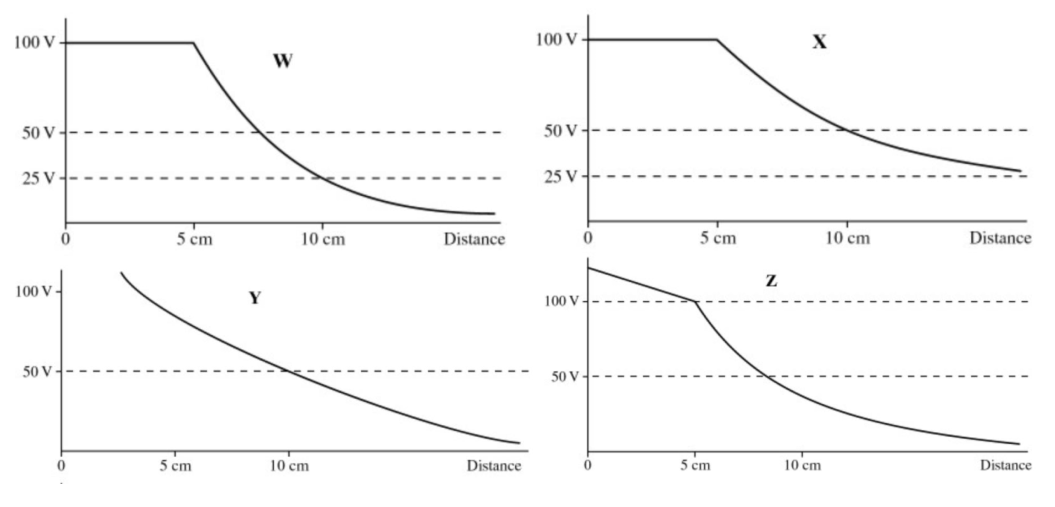
\includegraphics[scale=0.3]{figures/T4P2.png}
    \end{figure}
    
    \pause \begin{center}
        \textbf{Respuesta:} X.
    \end{center}
    
\end{frame}



\begin{frame}{Semana 5 (09/03/2023) - T4P3}
    
    \vspace{-1em}
    
    \begin{columns}
    \column{0.5\textwidth}
    El gráfico de la figura muestra la variación del potencial eléctrico $V(x)$ en función de la posición $x$.
    \column{0.4\textwidth}
    \begin{figure}
        \centering
        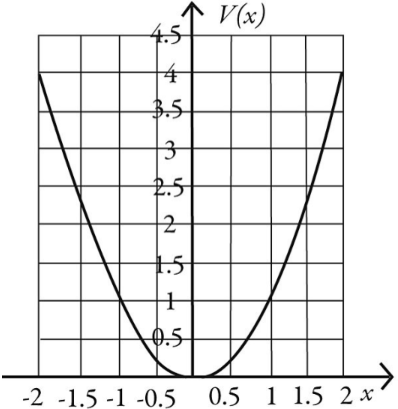
\includegraphics[scale=0.3]{figures/t4p3.png}
    \end{figure}
    \end{columns}
    
    \vspace{1em}
    
    ¿Cuál de las siguientes opciones describe correctamente la orientación de la componente $x$ del campo eléctrico a lo largo del eje $x$?
    
    \begin{itemize}
        \item[A)] $E_x$ es positivo desde $x = -2$ hasta $x = 2$.

        \item[B)] $E_x$ es positivo desde $x = -2$ hasta $x = 0$, y negativo desde $x = 0$ hasta $x = 2$.
        
        \item[C)] $E_x$ es negativo de $x = -2$ a $x = 0$, y positivo de $x = 0$ a $x = 2$.
        
        \item[D)] $E_x$ es negativo desde $x = -2$ hasta $x = 2$.
    \end{itemize}
    
    \pause \begin{center}
        \textbf{Respuesta:} B.
    \end{center}
    
\end{frame}

\begin{frame}{Semana 5 (09/03/2023) - T4P4}
    Una carga puntual de $+$4.0 $\mu$C y una carga puntual de $-$4,0 $\mu$C se colocan como se muestra en la figura. ¿Cuál es la diferencia de potencial, $V_A-V_B$, entre los puntos $A$ y $B$?
    
    \begin{figure}
        \centering
        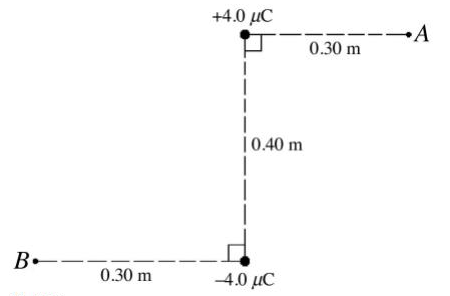
\includegraphics[scale=0.5]{figures/t4p4.png}
    \end{figure}
    
\end{frame}

\begin{frame}{Semana 5 (09/03/2023) - T4P5}
    The figure shows two arcs of a circle on which charges $+Q$ and $-Q$ have been spread uniformly. What is the value of the electric potential at the center of the circle?
    
    \begin{figure}
        \centering
        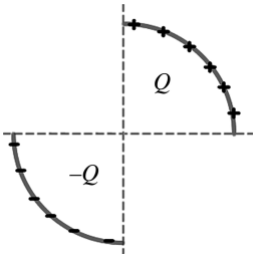
\includegraphics[scale=0.5]{figures/t4p5.png}
    \end{figure}
    
\end{frame}

\begin{frame}{Semana 5 (09/03/2023) - T4P6}
    Dos cargas puntuales de $+$1.0 $\mu$C y $-$2.0 $\mu$C están ubicadas a 0.50 m de distancia. ¿Cuál es la cantidad mínima de trabajo necesaria para separar las cargas y duplicar la distancia entre ellas?
    
    \begin{itemize}
        \item[A)] $-$36 mJ
        \item[B)] $+$18 mJ
        \item[C)]0 mJ
        \item[D)]$+$36 mJ
        \item[E)]$-$18 mJ
    \end{itemize}
    
    \pause \begin{center}
        \textbf{Respuesta:} B.
    \end{center}
    
\end{frame}

\begin{frame}{Semana 5 (09/03/2023) - T4P7}

        \begin{columns}
        \column{0.5\textwidth}
        La figura muestra una disposición de dos cargas de $-$4.5 nC, cada una separada por 5.0 mm de un protón. Si las dos cargas negativas se mantienen fijas en sus ubicaciones y al protón se le da una velocidad inicial $v$ como se muestra en la figura.
        \column{0.4\textwidth}
        \begin{figure}
        \centering
        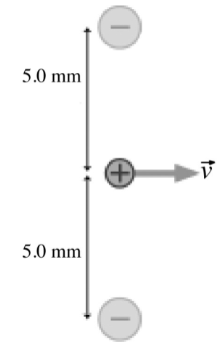
\includegraphics[scale=0.3]{figures/t4p7.png}
        \end{figure}
        \end{columns}
        
        \vspace{1em}
        
        ¿Cuál es la velocidad inicial mínima $v$ que necesita el protón para escapar totalmente de las cargas negativas?
        
        \begin{itemize}
        \item[A)] $1.8 \times 10^6$ m/s
        \item[B)] $3.5 \times 10^6$ m/s
        \item[C)] $6.8 \times 10^6$ m/s
        \item[D)] $1.4 \times 10^7$ m/s
        \end{itemize}
        
        \pause \centering \textbf{Respuesta:} A.
        
    \end{frame}

\begin{frame}{Semana 5 (09/03/2023) - Q4}
    Una carga $Q$ se distribuye uniformemente en un anillo de radio $a$. Una carga puntual $q$ está fija en el centro del anillo, como se muestra en la figura. Un electrón es lanzado desde el infinito hacia el anillo a lo largo del eje del anillo. Este electrón se detiene momentáneamente en un punto del eje que está a una distancia $d$ del centro del anillo. ¿Cuál es la velocidad inicial del electrón en el infinito?
    
    \begin{figure}
        \centering
        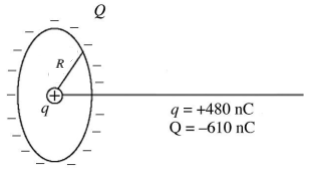
\includegraphics[scale=0.6]{figures/Q4.png}
    \end{figure}
    
\end{frame}